% https://wiki.physik.uzh.ch/cms/latex:tikz:arrows_to_nodes

% How to break text lines: https://tex.stackexchange.com/a/124114/173708

% Author: Izaak Neutelings (September 2018)
\documentclass[border=3pt,tikz]{standalone}
\usepackage{amsmath} % for \;
\usepackage{tikz}
\usepackage{xcolor}

\colorlet{myblue}{blue!70!black}
\colorlet{mylightblue}{blue!10}
\tikzset{>=latex} % for LaTeX arrow head

\begin{document}


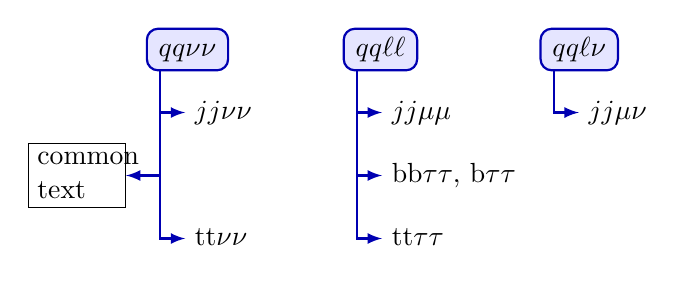
\begin{tikzpicture}[yscale=0.8,anchor=west]
  
  % FIRST COLUMN
  \node[anchor=west,draw=myblue,fill=mylightblue,thick,rounded corners=4,inner sep=1.5pt] (L) at (0,4) {\;\strut$qq\nu\nu$\;};  
  \node (L1) at (0.5,3) {\strut$jj\nu\nu$};
  \node (L2) at (-1.5,2) [draw, text width=1cm] {common text};   % break a line in two
  \node (L3) at (0.5,1) {\strut tt$\nu\nu$};
  \draw[->,myblue,thick] (L.south west) ++ (0.18,0) |- (L1.west);
  \draw[->,myblue,thick] (L.south west) ++ (0.18,0) |- (L2.east);
  \draw[->,myblue,thick] (L.south west) ++ (0.18,0) |- (L3.west);
  
  % SECOND COLUMN
  \begin{scope}[shift={(2.5,0)}]
    \node[draw=myblue,fill=mylightblue,thick,rounded corners=4,inner sep=1.5pt] (M) at (0,4) {\;\strut$qq\ell\ell$\;};
    \node (M1) at (0.5,3) {\strut$jj\mu\mu$};
    \node (M2) at (0.5,2) {\strut bb$\tau\tau$, b$\tau\tau$};
    \node (M3) at (0.5,1) {\strut tt$\tau\tau$};
    \draw[->,myblue,thick] (M.south west)++(0.18,0) |- (M1.west);
    \draw[->,myblue,thick] (M.south west)++(0.18,0) |- (M2.west);
    \draw[->,myblue,thick] (M.south west)++(0.18,0) |- (M3.west);
  \end{scope}
  
  % THIRD COLUMN
  \begin{scope}[shift={(5.0,0)}]
    \node[draw=myblue,fill=mylightblue,thick,rounded corners=4,inner sep=1.5pt] (R) at (0,4) {\;\strut$qq\ell\nu$\;};
    \node (R1) at (0.5,3) {\strut$jj\mu\nu$};
    \draw[->,myblue,thick] (R.south west)++(0.18,0) |- (R1.west);
  \end{scope}

\end{tikzpicture}


\end{document}